\part{The \LaTeX\ standard class}
\parindent0pt
\setlength\columnsep{2em}
\def\Paragraph#1{{\bf #1}\quad}
\chapter{The book.cls}
\clearpage

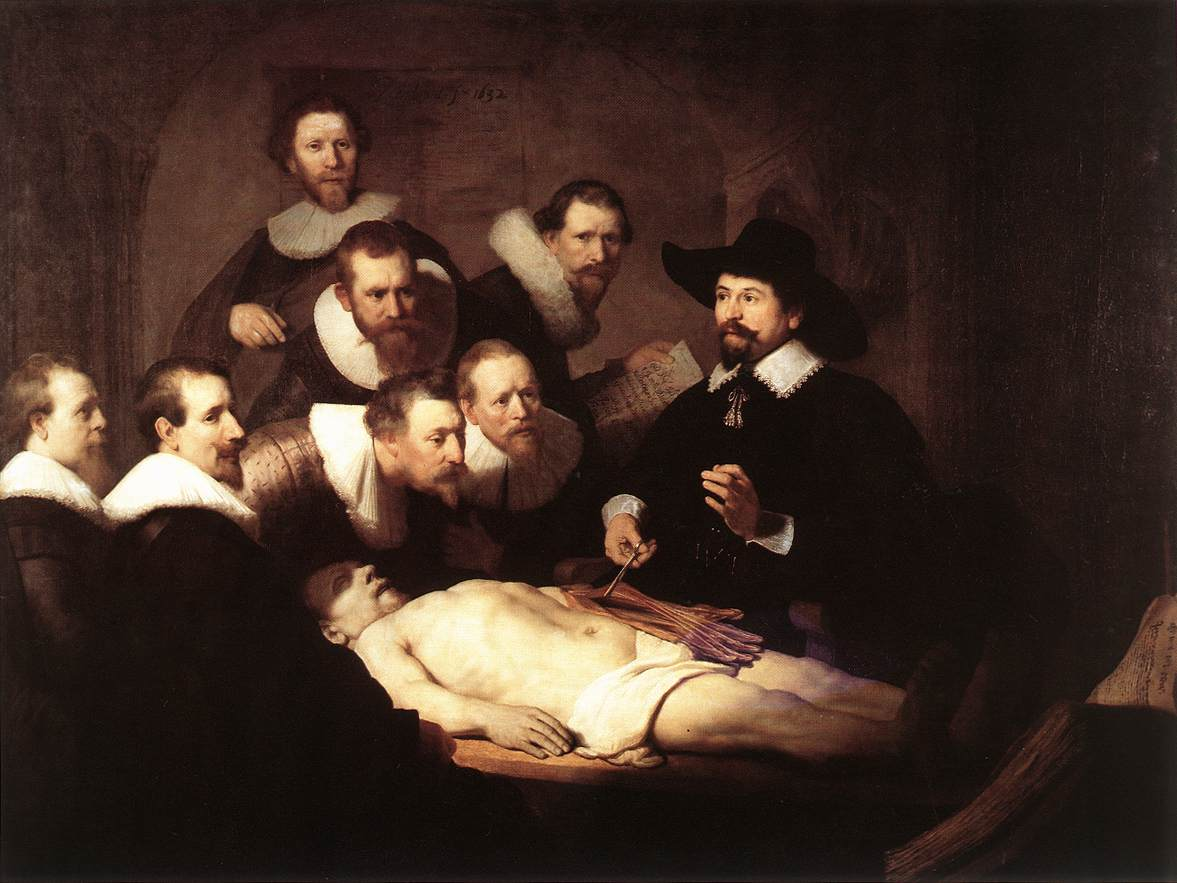
\includegraphics[width=\textwidth]{./graphics/anatomy}

\vspace{2\baselineskip}

\textbf{\Large DISSECTING THE BOOK CLASS}

\begin{multicols}{2}
This appendix describes the listing of the book class as defined by \latex. It is described here with extra commentary in order to enable you to understand, how it all works.

\lipsum[1-3]
\end{multicols}

\section{GENERAL}

\begin{multicols}{2}
The book class starts normally with declaring the version of LaTeX, required
and naming the class it provides. The class choices are always checked for backward compatibility with the earlier version of \latex. All commands that need to be modified between two column and one column layouts, check the setting and branch accordingly. Another primary choice is if the book is to be printed on both sides or only on one side.
\end{multicols}


\begin{teX}
\NeedsTeXFormat{LaTeX2e}[1995/12/01]
\ProvidesClass{book}
              [2007/10/19 v1.4h
 Standard LaTeX document class]
\end{teX}


\begin{teX}
\newcommand\@ptsize{}
\newif\if@restonecol
\newif\if@titlepage
\@titlepagetrue
\newif\if@openright
\newif\if@mainmatter \@mainmattertrue
\end{teX}

\begin{multicols}{2}
\Paragraph{Paper size.} After checking for compatibilty with older versions the code branches to define the different standard paper sizes! The options that are declared are, |a4paper|, |a5paper|, | b5paper|, |letterpaper|, |legalpaper| and  |executivepaper|. The class will then later on process the options and set the default to |letterpaper|. \footnote{The package \texttt{geometry}, some classes such as the Octavo and KOMA classes add additional sizes to cater for other standards.}
\end{multicols}
\begin{teX}
\if@compatibility\else
\DeclareOption{a4paper}
   {\setlength\paperheight {297mm}%
    \setlength\paperwidth  {210mm}}
\DeclareOption{a5paper}
   {\setlength\paperheight {210mm}%
    \setlength\paperwidth  {148mm}}
\DeclareOption{b5paper}
   {\setlength\paperheight {250mm}%
    \setlength\paperwidth  {176mm}}
\DeclareOption{letterpaper}
   {\setlength\paperheight {11in}%
    \setlength\paperwidth  {8.5in}}
\DeclareOption{legalpaper}
   {\setlength\paperheight {14in}%
    \setlength\paperwidth  {8.5in}}
\DeclareOption{executivepaper}
   {\setlength\paperheight {10.5in}%
    \setlength\paperwidth  {7.25in}}
\end{teX}

\begin{multicols}{2}
\Paragraph{Paper orientation.} the paper orientation is set based on the |landscape| option. If it is declared it stores the |\paperheight| into one of the \latex kernel scratch registers, |\@tempdima| and then reverses the length with the |\paperwidth|.
\end{multicols}

\begin{teX}
\DeclareOption{landscape}
   {\setlength\@tempdima   {\paperheight}%
    \setlength\paperheight {\paperwidth}%
    \setlength\paperwidth  {\@tempdima}}
\fi
\end{teX}

\begin{multicols}{2}
\Paragraph{Font sizing} The class provides three font sizes |10pt|, |11pt| and |12pt|. It default to ten point text.
\end{multicols}

\begin{teX}
\if@compatibility
  \renewcommand\@ptsize{0}
\else
\DeclareOption{10pt}{\renewcommand\@ptsize{0}}
\fi
\DeclareOption{11pt}{\renewcommand\@ptsize{1}}
\DeclareOption{12pt}{\renewcommand\@ptsize{2}}
\end{teX}

\begin{multicols}{2}
\Paragraph{Recto and verso pages.} The class provides the |oneside| and |twoside| options for switching between one side printing or two side printing.  It sets the booleans |\if@twoside| and |\if@mparswitch| accordingly. These booleans are used later on for setting other variables.
\end{multicols}
\begin{teX}
\if@compatibility\else
\DeclareOption{oneside}{\@twosidefalse \@mparswitchfalse}
\fi
\DeclareOption{twoside}{\@twosidetrue  \@mparswitchtrue}
\end{teX}

\begin{multicols}{2}
\Paragraph{Draft and final options.} The options draft and final, just set the |\overfullrule| to either 1pt or 0pt. The |\overfullrule| is a \tex command and simply prints a small vertical line to indicate overfull boxes for the attention of the author. 
\end{multicols}

\begin{teX}
\DeclareOption{draft}{\setlength\overfullrule{5pt}}
\if@compatibility\else
\DeclareOption{final}{\setlength\overfullrule{0pt}}
\fi
\end{teX}

\begin{multicols}{2}
\Paragraph{Title page option.} If the book class, needed such an option is debatable. The |titlepage| option is normally set as true and results in the title being on its own page. The |notitlepage| will omit the page break and display the title on the same page with that of the opening text. Highly unlikely for any author to use it for a book. It is useful for the article class.
\end{multicols}

\begin{teX}
\DeclareOption{titlepage}{\@titlepagetrue}
\if@compatibility\else
\DeclareOption{notitlepage}{\@titlepagefalse}
\fi
\end{teX}

\begin{multicols}{2}
\Paragraph{Display of chapters.} Chapters can be set to start only on an even page or any page. The class provides the options |openright| and |openany|.
\end{multicols}


\begin{teX}
\if@compatibility
\@openrighttrue
\else
\DeclareOption{openright}{\@openrighttrue}
\DeclareOption{openany}{\@openrightfalse}
\fi
\end{teX}


\begin{teX}
\if@compatibility\else
\DeclareOption{onecolumn}{\@twocolumnfalse}
\fi
\DeclareOption{twocolumn}{\@twocolumntrue}
\DeclareOption{leqno}{\input{leqno.clo}}
\DeclareOption{fleqn}{\input{fleqn.clo}}
\DeclareOption{openbib}{%
  \AtEndOfPackage{%
   \renewcommand\@openbib@code{%
      \advance\leftmargin\bibindent
      \itemindent -\bibindent
      \listparindent \itemindent
      \parsep \z@
      }%
   \renewcommand\newblock{\par}}%
}
\end{teX}

We now execute the options and process them.
\begin{teX}
\ExecuteOptions{letterpaper,10pt,twoside,onecolumn,final,openright}
\ProcessOptions
\end{teX}

\begin{multicols}{2}
\textbf{The .clo files}\quad The book class now inputs the file .clo etc that defines the fontsizes
 for anything specific to the 10pt. These files hold quite a bit of information and size related commands for the
standard sizes provided by \latex. The |.clo| files also set many other parameters for page sizing, lists, paper sectioning, such as margins, marginpars and the like.
\end{multicols}

\begin{teX}
\input{bk1\@ptsize.clo}
\setlength\lineskip{1\p@}
\setlength\normallineskip{1\p@}
\renewcommand\baselinestretch{}
\setlength\parskip{0\p@ \@plus \p@}
\end{teX}

\begin{multicols}{2}
\Paragraph{Penalties.} Here the following penalties are set.
\end{multicols}

\begin{teX}
\@lowpenalty   51
\@medpenalty  151
\@highpenalty 301
\end{teX}

\begin{multicols}{2}
\textbf{Float control parameters.}\quad The allowable number of floats on a page are controlled by a number of parameters. These are set here. Many users overwrite these parameters in order to have more control on the placement of floats.
\end{multicols}


\begin{teX}
\setcounter{topnumber}{2}
\renewcommand\topfraction{.7}
\setcounter{bottomnumber}{1}
\renewcommand\bottomfraction{.3}
\setcounter{totalnumber}{3}
\renewcommand\textfraction{.2}
\renewcommand\floatpagefraction{.5}
\setcounter{dbltopnumber}{2}
\renewcommand\dbltopfraction{.7}
\renewcommand\dblfloatpagefraction{.5}
\end{teX}

\begin{multicols}{2}
\textbf{Running head and foot.}\quad A page header or simply header in typography is text which is separated from the main body of text and appears at the top of a printed page. Word processing programs usually provide for the creation and maintenance of page headers, which are often the same from page to page, with merely small differences in information, such as page number.

In publishing, the page header (or ``pagehead'') is often referred to as the running head. Typical running heads in a book might consist of the book title on the left-hand (verso) page, and the chapter title on the right-hand (recto) page, or chapter title on the verso and subsection title on the recto.
\end{multicols}


\begin{teX}
\if@twoside
  \def\ps@headings{%
      \let\@oddfoot\@empty\let\@evenfoot\@empty
      \def\@evenhead{\thepage\hfil\slshape\leftmark}%
      \def\@oddhead{{\slshape\rightmark}\hfil\thepage}%
      \let\@mkboth\markboth
 % chapter
  \def\chaptermark##1{%
      \markboth {\MakeUppercase{%
        \ifnum \c@secnumdepth >\m@ne
          \if@mainmatter
            \@chapapp\ \thechapter. \ %
          \fi
        \fi
        ##1}}{}}%
% section
    \def\sectionmark##1{%
      \markright {\MakeUppercase{%
        \ifnum \c@secnumdepth >\z@
          \thesection. \ %
        \fi
        ##1}}}}
\else
  \def\ps@headings{%
    \let\@oddfoot\@empty
    \def\@oddhead{{\slshape\rightmark}\hfil\thepage}%
    \let\@mkboth\markboth
    \def\chaptermark##1{%
      \markright {\MakeUppercase{%
        \ifnum \c@secnumdepth >\m@ne
          \if@mainmatter
            \@chapapp\ \thechapter. \ %
          \fi
        \fi
        ##1}}}}
\fi
\def\ps@myheadings{%
    \let\@oddfoot\@empty\let\@evenfoot\@empty
    \def\@evenhead{\thepage\hfil\slshape\leftmark}%
    \def\@oddhead{{\slshape\rightmark}\hfil\thepage}%
    \let\@mkboth\@gobbletwo
    \let\chaptermark\@gobble
    \let\sectionmark\@gobble
    }
\end{teX}

\begin{multicols}{2}\index{headings!plain}
Please note the \textit{plain} headings are not defined in the class. These are defined in the \latex kernel\footnote{See \texttt{File J: ltpage.dtx}, page 312.}

\begin{Code}
\ps@plain The plain page style: No head, centred page number in foot.
13 \def\ps@plain{\let\@mkboth\@gobbletwo
14 \let\@oddhead\@empty\def\@oddfoot{\reset@font\hfil\thepage
15 \hfil}\let\@evenhead\@empty\let\@evenfoot\@oddfoot}
\end{Code}



\textbf{Title pages.}\quad Title pages are defined between a conditional, that handle the option |titlepage|
and. The commands just take mostly of the typography. If you use the option |notitlepage| in the book class, the title will be similar for all practical purposes to that of an |article| and it will appear on the top of the first page.

The |\maketitle| sets the |\footnotesise|, the |\footnoterule| and the |\footnote|.
\end{multicols}

\begin{teX}
 \if@titlepage
  \newcommand\maketitle{\begin{titlepage}%
  \let\footnotesize\small
  \let\footnoterule\relax
  \let \footnote \thanks
  \null\vfil
  \vskip 60\p@
  \begin{center}%
    {\LARGE \@title \par}%
    \vskip 3em%
    {\large
     \lineskip .75em%
      \begin{tabular}[t]{c}%
        \@author
      \end{tabular}\par}%
      \vskip 1.5em%
    {\large \@date \par}%       % Set date in \large size.
  \end{center}\par
  \@thanks
  \vfil\null
  \end{titlepage}%
  \setcounter{footnote}{0}%
  \global\let\thanks\relax
  \global\let\maketitle\relax
  \global\let\@thanks\@empty
  \global\let\@author\@empty
  \global\let\@date\@empty
  \global\let\@title\@empty
  \global\let\title\relax
  \global\let\author\relax
  \global\let\date\relax
  \global\let\and\relax
}
\else
\newcommand\maketitle{\par
  \begingroup
    \renewcommand\thefootnote{\@fnsymbol\c@footnote}%
    \def\@makefnmark{\rlap{\@textsuperscript{\normalfont\@thefnmark}}}%
    \long\def\@makefntext##1{\parindent 1em\noindent
            \hb@xt@1.8em{%
                \hss\@textsuperscript{\normalfont\@thefnmark}}##1}%
    \if@twocolumn
      \ifnum \col@number=\@ne
        \@maketitle
      \else
        \twocolumn[\@maketitle]%
      \fi
    \else
      \newpage
      \global\@topnum\z@   % Prevents figures from going at top of page.
      \@maketitle
    \fi
    \thispagestyle{plain}\@thanks
  \endgroup
  \setcounter{footnote}{0}%
  \global\let\thanks\relax
  \global\let\maketitle\relax
  \global\let\@maketitle\relax
  \global\let\@thanks\@empty
  \global\let\@author\@empty
  \global\let\@date\@empty
  \global\let\@title\@empty
  \global\let\title\relax
  \global\let\author\relax
  \global\let\date\relax
  \global\let\and\relax
}
\def\@maketitle{%
  \newpage
  \null
  \vskip 2em%
  \begin{center}%
  \let \footnote \thanks
    {\LARGE \@title \par}%
    \vskip 1.5em%
    {\large
      \lineskip .5em%
      \begin{tabular}[t]{c}%
        \@author
      \end{tabular}\par}%
    \vskip 1em%
    {\large \@date}%
  \end{center}%
  \par
  \vskip 1.5em}
\fi
\end{teX}

\begin{multicols}{2}
\textbf{Section counters.}\quad 
In LaTeX all defaults all document section are numbered by default. These numbers are kept in counters, named after the section name. A series of commands are provided to access these numbers.
All the counters are in arabic numerals, with the exception of "part", which is in Roman.
\end{multicols}

\begin{teX}
\newcommand*\chaptermark[1]{}
\setcounter{secnumdepth}{2}
\newcounter {part}
\newcounter {chapter}
\newcounter {section}[chapter]
\newcounter {subsection}[section]
\newcounter {subsubsection}[subsection]
\newcounter {paragraph}[subsubsection]
\newcounter {subparagraph}[paragraph]
\renewcommand \thepart {\@Roman\c@part}
\renewcommand \thechapter {\@arabic\c@chapter}
\renewcommand \thesection {\thechapter.\@arabic\c@section}
\renewcommand\thesubsection   {\thesection.\@arabic\c@subsection}
\renewcommand\thesubsubsection{\thesubsection.\@arabic\c@subsubsection}
\renewcommand\theparagraph    {\thesubsubsection.\@arabic\c@paragraph}
\renewcommand\thesubparagraph {\theparagraph.\@arabic\c@subparagraph}
\newcommand\@chapapp{\chaptername}
\end{teX}

\begin{multicols}{2}
\textbf{Frontmatter, mainmatter and backmatter.} These are author command to set mostly, the page numbering and the clearing of pages for two page layouts. Front matter has lower roman pages numbering and the main matter has arabic numerals.
\end{multicols}

\emphasis{frontmatter,mainmatter,backmatter}
\begin{teXXX}
\newcommand\frontmatter{%
    \cleardoublepage
  \@mainmatterfalse
  \pagenumbering{roman}}

\newcommand\mainmatter{%
    \cleardoublepage
  \@mainmattertrue
  \pagenumbering{arabic}}

\newcommand\backmatter{%
  \if@openright
    \cleardoublepage
  \else
    \clearpage
  \fi
  \@mainmatterfalse}
\end{teXXX}

\begin{multicols}{2}
\Paragraph{Part.}The is the definition of part. The Part is displayed with a plain header and the it goes into the secdef. If the section depth is greater or equal -2, the start counter is increased and the part is added to the toc, using |\addcontentsline|. 
The partname i.e., default 'Part' gets printer either way except for the star version of the command.
\end{multicols}

\emphasis{@part,@spart,secdef}
\begin{teXXX}
\newcommand\part{%
  \if@openright
    \cleardoublepage
  \else
    \clearpage
  \fi
  \thispagestyle{plain}%
  \if@twocolumn
    \onecolumn
    \@tempswatrue
  \else
    \@tempswafalse
  \fi
  \null\vfil
  \secdef\@part\@spart}
\end{teXXX}

\begin{multicols}{2}
 The important command to remember here
is |\secdef|. This is defined in the kernel and not in the classes \texttt{ltsect.dtx}. Essentially in the code |\@part| calls the unstar command and the @spart calls the starred command. We copy the definition from the kernel for convenience.
\end{multicols}

\begin{teXXX}
is \secdef{unstarcmds}{unstarcmds}{starcmds}
When defining a \chapter or \section command without using \@startsection,
you can use \secdef as follows:
1. \def\chapter{ . . . \secdef \starcmd \unstarcmd}
2. \def\hstarcmdi[#1]#2{ . . . } % Command to define \chapter[. . . ]{. . . }
3. \def\unstarcmd#1{ . . . } % Command to define \chapter*{. . . }
125 \def\secdef#1#2{\@ifstar{#2}{\@dblarg{#1}}}
\end{teXXX}

The |@part| starts now,

\begin{teXXX}
\def\@part[#1]#2{%
    \ifnum \c@secnumdepth >-2\relax
      \refstepcounter{part}%
      \addcontentsline{toc}{part}{\thepart\hspace{1em}#1}%
    \else
      \addcontentsline{toc}{part}{#1}%
    \fi
    \markboth{}{}%
    {\centering
     \interlinepenalty \@M
     \normalfont
     \ifnum \c@secnumdepth >-2\relax
       \huge\bfseries \partname\nobreakspace\thepart
       \par
       \vskip 20\p@
     \fi
     \Huge \bfseries #2\par}%
    \@endpart}
\end{teXXX}

\begin{multicols}{2}
The starred version of the command is provided next. The difference the name `Part'' is not displayed. However the parameter provided by the user is displayed. A normal font is provided. Final settings depending on @openright and header styles are set and the code macro is completed.
\end{multicols}

\begin{teXXX}
\def\@spart#1{%
    {\centering
     \interlinepenalty \@M
     \normalfont
     \Huge \bfseries #1\par}%
    \@endpart}

\def\@endpart{\vfil\newpage
              \if@twoside
               \if@openright
                \null
                \thispagestyle{empty}%
                \newpage
               \fi
              \fi
              \if@tempswa
                \twocolumn
              \fi}
\end{teXXX}

\begin{multicols}{2}
\Paragraph{Chapter}. The chapter definition follows, the same pattern as that of the part definitions. It calls secdef and defines commands for the starred and unstarred versions.
\end{multicols}

\begin{teXXX}
\newcommand\chapter{\if@openright\cleardoublepage\else\clearpage\fi
                    \thispagestyle{plain}%
                    \global\@topnum\z@
                    \@afterindentfalse
                    \secdef\@chapter\@schapter}
\end{teXXX}

\Paragraph{Unstarred version}

\begin{teXXX}
\def\@chapter[#1]#2{\ifnum \c@secnumdepth >\m@ne
                       \if@mainmatter
                         \refstepcounter{chapter}%
                         \typeout{\@chapapp\space\thechapter.}%
                         \addcontentsline{toc}{chapter}%
                                   {\protect\numberline{\thechapter}#1}%
                       \else
                         \addcontentsline{toc}{chapter}{#1}%
                       \fi
                    \else
                      \addcontentsline{toc}{chapter}{#1}%
                    \fi
                    \chaptermark{#1}%
                    \addtocontents{lof}{\protect\addvspace{10\p@}}%
                    \addtocontents{lot}{\protect\addvspace{10\p@}}%
                    \if@twocolumn
                      \@topnewpage[\@makechapterhead{#2}]%
                    \else
                      \@makechapterhead{#2}%
                      \@afterheading
                    \fi}
\end{teXXX}

\begin{multicols}{2}
\Paragraph{Defining the looks of the Chapter heading.}

Good practice dictates, that when you change the chapterhead layout for the numbered version, you also change it for the star version of the command. You can do that by using two different macros, although at first glance it might be difficult to see where the difference is.
\end{multicols}


\emphasis{@makeschapterhead,@makechapterhead}
\begin{teXXX}
\def\@makechapterhead
\def\@makeschapterhead
\end{teXXX}

\begin{teXXX}
\def\@makechapterhead#1{%
  \vspace*{50\p@}%
  {\parindent \z@ \raggedright \normalfont
    \ifnum \c@secnumdepth >\m@ne
      \if@mainmatter
        \huge\bfseries \@chapapp\space \thechapter
        \par\nobreak
        \vskip 20\p@
      \fi
    \fi
    \interlinepenalty\@M
    \Huge \bfseries #1\par\nobreak
    \vskip 40\p@
  }}
\end{teXXX}

\begin{multicols}{2}
Finally the starred version of the command is called. This now checks for twocolumn or one column via an if statement and executes, the makeschapterhead. Another mysterious and wonderful command appears again from the LaTeX source2e. `\@afterheading`. This command 
is just a hook for custom headings? (Needs to be reviewed again).
\end{multicols}

\begin{teXXX}
\def\@schapter#1{\if@twocolumn
                   \@topnewpage[\@makeschapterhead{#1}]%
                 \else
                   \@makeschapterhead{#1}%
                   \@afterheading
                 \fi}
\end{teXXX}

And finally the amkeschapterhead (remember s for star).

\begin{teXXX}
\def\@makeschapterhead#1{%
  \vspace*{50\p@}%
  {\parindent \z@ \raggedright
    \normalfont
    \interlinepenalty\@M
    \Huge \bfseries  #1\par\nobreak
    \vskip 40\p@
  }}
\end{teXXX}

All sorts of variations of the above two commands can be found in different classes, such as |KOMA|, |memoir| and others. The example which follows, typesets the headings as shown in \fref{fig:chapterhead-17}. The |@makechapterhead| command is modified to produce a centered heading which is displayed between two heavy rules. This style can be found in quite a number of books.

\begin{figure*}[htbp]
\includegraphics[width=\linewidth]{./graphics/chapterhead-17}
\caption{Modifying the way the chapterhead looks can be achieved by redefining the \texttt{\textbackslash @makechapterhead} and \texttt{\textbackslash @makeschapterhead} commands.}
\label{fig:chapterhead-17}
\end{figure*}

\section*{Full working example}

\begin{teX}
\documentclass[oneside]{book}
\usepackage[english]{babel}
\usepackage{lipsum}
\makeatletter
\def\thickhrule{\leavevmode \leaders \hrule height 1ex \hfill \kern \z@}

%% Note the difference between the commands the one is 
%% make and the other one is makes
\renewcommand{\@makechapterhead}[1]{%
  \vspace*{10\p@}%
  {\parindent \z@ \centering \reset@font
        {\Huge \scshape  \thechapter }
        \par\nobreak
        \vspace*{10\p@}%
        \interlinepenalty\@M
        \thickhrule
        \par\nobreak
        \vspace*{2\p@}%
        {\Huge \bfseries #1\par\nobreak}
        \par\nobreak
        \vspace*{2\p@}%
        \thickhrule
    \vskip 40\p@
    \vskip 100\p@
  }}

%% This is makes
\def\@makeschapterhead#1{%
  \vspace*{10\p@}%
  {\parindent \z@ \centering \reset@font
        {\Huge \scshape \vphantom{\thechapter}}
        \par\nobreak
        \vspace*{10\p@}%
        \interlinepenalty\@M
        \thickhrule
        \par\nobreak
        \vspace*{2\p@}%
        {\Huge \bfseries #1\par\nobreak}
        \par\nobreak
        \vspace*{2\p@}%
        \thickhrule
    \vskip 100\p@
  }}
\begin{document}
\chapter{The Real Numbers}
\lipsum[1-2]
\chapter*{The Imaginary Numbers}
\lipsum[1-2]
\end{document}
\end{teX}

\begin{multicols}{2}
\Paragraph{The sections.}
In this section, all the document elements besides the Chapter and the Part are Defined. They use the mother of all commands from the kernel
ltsection.dtx, named |\@startsection|. This is just a call to the kernel command. No other settings are done here. In order to remember what it does we refer to its definition in the kernel. Of interest is the sixth argument which sets the style.
The parameter takes eight parameters, some of them optional. We discuss this command in more detail in the kernel chapter.

\end{multicols}


\begin{teX}
\newcommand\section{\@startsection {section}{1}{\z@}%
                                   {-3.5ex \@plus -1ex \@minus -.2ex}%
                                   {2.3ex \@plus.2ex}%
                                   {\normalfont\Large\bfseries}}
\newcommand\subsection{\@startsection{subsection}{2}{\z@}%
                                     {-3.25ex\@plus -1ex \@minus -.2ex}%
                                     {1.5ex \@plus .2ex}%
                                     {\normalfont\large\bfseries}}
\newcommand\subsubsection{\@startsection{subsubsection}{3}{\z@}%
                                     {-3.25ex\@plus -1ex \@minus -.2ex}%
                                     {1.5ex \@plus .2ex}%
                                     {\normalfont\normalsize\bfseries}}
\newcommand\paragraph{\@startsection{paragraph}{4}{\z@}%
                                    {3.25ex \@plus1ex \@minus.2ex}%
                                    {-1em}%
                                    {\normalfont\normalsize\bfseries}}
\newcommand\subparagraph{\@startsection{subparagraph}{5}{\parindent}%
                                       {3.25ex \@plus1ex \@minus .2ex}%
                                       {-1em}%
                                      {\normalfont\normalsize\bfseries}}
\if@twocolumn
  \setlength\leftmargini  {2em}
\else
  \setlength\leftmargini  {2.5em}
\fi
\leftmargin  \leftmargini
\setlength\leftmarginii  {2.2em}
\setlength\leftmarginiii {1.87em}
\setlength\leftmarginiv  {1.7em}
\if@twocolumn
  \setlength\leftmarginv  {.5em}
  \setlength\leftmarginvi {.5em}
\else
  \setlength\leftmarginv  {1em}
  \setlength\leftmarginvi {1em}
\fi
\setlength  \labelsep  {.5em}
\setlength  \labelwidth{\leftmargini}
\addtolength\labelwidth{-\labelsep}
\@beginparpenalty -\@lowpenalty
\@endparpenalty   -\@lowpenalty
\@itempenalty     -\@lowpenalty
\renewcommand\theenumi{\@arabic\c@enumi}
\renewcommand\theenumii{\@alph\c@enumii}
\renewcommand\theenumiii{\@roman\c@enumiii}
\renewcommand\theenumiv{\@Alph\c@enumiv}
\newcommand\labelenumi{\theenumi.}
\newcommand\labelenumii{(\theenumii)}
\newcommand\labelenumiii{\theenumiii.}
\newcommand\labelenumiv{\theenumiv.}
\renewcommand\p@enumii{\theenumi}
\renewcommand\p@enumiii{\theenumi(\theenumii)}
\renewcommand\p@enumiv{\p@enumiii\theenumiii}
\newcommand\labelitemi{\textbullet}
\newcommand\labelitemii{\normalfont\bfseries \textendash}
\newcommand\labelitemiii{\textasteriskcentered}
\newcommand\labelitemiv{\textperiodcentered}
\newenvironment{description}
               {\list{}{\labelwidth\z@ \itemindent-\leftmargin
                        \let\makelabel\descriptionlabel}}
               {\endlist}
\newcommand*\descriptionlabel[1]{\hspace\labelsep
                                \normalfont\bfseries #1}
\end{teX}

\begin{multicols}{2}
\textbf{The verse environment}\quad \latex's verse environment, can only serve for the incidental use of a few stanzas. It leaves most of the formatting to the author.  It redefines the line break |\\| to a |\centercr|.
\end{multicols}

\begin{teX}
\newenvironment{verse}
    {\let\\\@centercr(*@\protect\footnote{This is defined in ltmiscen.dtx}@*)
     \list{}{\itemsep  \z@
             \itemindent   -1.5em%
             \listparindent\itemindent
             \rightmargin  \leftmargin
             \advance\leftmargin 1.5em}%
       \item\relax}
    {\endlist}
\end{teX}
\makeatletter
\newenvironment{Verse}
    {\let\\\@centercr%
     \list{}{\itemsep1pt
             \itemindent-1.5em%
             \listparindent\itemindent
             \rightmargin\leftmargin
             \advance\leftmargin 1.5em}%
       \item\relax}
    {\endlist}
\makeatother
\begin{Verbatim}
  \begin{Verse}
     My mobile test\\
     this is other\\
     this is last\\
  \end{Verse}
\end{Verbatim}
The environment doesn't really do much, the way I see it but just move the poem a couple of ems inwards 
to much the definition of lists. Most people will want more from a poem environment.
\begin{Verse}
     My mobile test\\
      this is other\\
       this is last\\
\end{Verse}

The simplest thing we can add to this environment if we want to modify it, is a hook. This we can do using the |blckcntrl| package. \sidenote{From the \url{http://www.ifi.uio.no/it/latex-links/blkcntrl.pdf}}.

\begin{teX}
\renewenvironment{verse}
50 {\let\\\@centercr
51 \relax\list{}{\setlength{\itemsep}{\z@}%
52 \setlength{\itemindent}{-1.5em}%
53 \setlength{\listparindent}{\itemindent}%
54 \setlength{\rightmargin}{\leftmargin}%
55 \addtolength{\leftmargin}{1.5em}}%
56 \item\relax\PreVerse\relax}
57 {\endlist}
\end{teX}

Using the command |\PreVerse|, we can add a block at the beginning of the block. For example some code to make a poem title and insert it later on. The setting of the rightmargin to the leftmargin here is curious. It might for example give us problems with |tufte-latex| classes.

\begin{multicols}{2}
\textbf{The quote and quotation environments.}\quad The environments |quote| and |quotation| are defined next. Again they are defined using the general |\list| environment. Again the general |\list|, is used in the definition. The |listparindent| is set to 1.5 em.
\end{multicols}

\begin{teX}
\newenvironment{quotation}
               {\list{}{\listparindent 1.5em%
                        \itemindent\listparindent
                        \rightmargin\leftmargin
                        \parsep\z@ \@plus\p@}%
                \item\relax}
               {\endlist}
\end{teX}

\begin{teX}
\newenvironment{quote}
               {\list{}{\rightmargin\leftmargin}%
                \item\relax}
               {\endlist}




\section{The \protect\texttt{titlepage} environment}
\if@compatibility
\newenvironment{titlepage}
    {%
      \cleardoublepage
      \if@twocolumn
        \@restonecoltrue\onecolumn
      \else
        \@restonecolfalse\newpage
      \fi
      \thispagestyle{empty}%
      \setcounter{page}\z@
    }%
    {\if@restonecol\twocolumn \else \newpage \fi
    }
\else
\newenvironment{titlepage}
    {%
      \cleardoublepage
      \if@twocolumn
        \@restonecoltrue\onecolumn
      \else
        \@restonecolfalse\newpage
      \fi
      \thispagestyle{empty}%
      \setcounter{page}\@ne
    }%
    {\if@restonecol\twocolumn \else \newpage \fi
     \if@twoside\else
        \setcounter{page}\@ne
     \fi
    }
\fi
\end{teX}



\begin{multicols}{2}
\includegraphics[width=\linewidth]{./graphics/appendix}

\Paragraph{The Appendix.}
Similarly to the chapter sectioning commands, the Appendix is not defined as a section. It simply sets the chapter and section counters to zero and sets the name of the section. All the relevant counters and uses letters for the numbering of the following chapters etc. If you closely follow the code, it is all based on the chapter command, except that it defaults to Alphanumeric counting.

\begin{teX}
\newcommand\appendix{\par
  \setcounter{chapter}{0}%
  \setcounter{section}{0}%
  \gdef\@chapapp{\appendixname}(*@\sidenote{The actual literal used for \textbackslash{appendixname} is defined later on, so that you can customize the language}\label{appendixname}@*)
  \gdef\thechapter{\@Alph\c@chapter}}
\end{teX}

An Appendix page has the same looks and feel to that of a Chapter. For all practical purposes, it is a chapter, with different labels and roman numbering.
\end{multicols}

\begin{multicols}{2}
\Paragraph{General Settings.} Here, some general settings are set. These include settings for framed boxes, tabbing separators and array column separators.

\end{multicols}
\begin{teX}
\setlength\arraycolsep{5\p@}
\setlength\tabcolsep{6\p@}
\setlength\arrayrulewidth{.4\p@}
\setlength\doublerulesep{2\p@}
\setlength\tabbingsep{\labelsep}
\skip\@mpfootins = \skip\footins
\setlength\fboxsep{3\p@}
\setlength\fboxrule{.4\p@}
\end{teX}

\begin{multicols}{2}
\Paragraph{Equation numbering}
The equation counter is reset according to the chapter counter, using the \latex kernel command |\@addtoreset|. 

\end{multicols}
\begin{teX}
\@addtoreset {equation}{chapter}
\renewcommand\theequation
  {\ifnum \c@chapter>\z@ \thechapter.\fi \@arabic\c@equation}
\end{teX}

\section*{FIGURE AND TABLE ENVIRONMENTS}

\begin{multicols}{2}
\Paragraph{Figure Environment} The figure environment is defined using commands that have been provided by the kernel.  The command |\thefigure| is first redefined to display the combination of the chapter dot figure counter, all in arabic numerals. The extension for the list of figures and finally the floats for single column and double column.

\end{multicols}


\begin{teX}
\newcounter{figure}[chapter]
\renewcommand \thefigure
     {\ifnum \c@chapter>\z@ \thechapter.\fi \@arabic\c@figure}
\end{teX}

\begin{macro}{\fps@figure} This macro is required by the output routine. It defines the
default placement specifiers for the figure environment. For many authors this is not
satisfactory without the `h' option.

\begin{teX}
\def\fps@figure{tbp}
\end{teX}
\end{macro}

\begin{macro}{\ftype@figure} Note here that this is a number. Each float number is defined
as to type power 2. The environment uses |\@float| and |\end@float| from the float.dtx class (see
Line \ref{float}} in the kernel. It is of interest that the optional argument of the figure environment
gets passed to |\@float{type}[placement]|. This gets redefined in the |float| class, if an optional
parameter has been set.

\begin{teX}
\def\ftype@figure{1}
\def\ext@figure{lof}
\def\fnum@figure{\figurename\nobreakspace\thefigure}
\newenvironment{figure}
               {\@float{figure}}
               {\end@float}
\newenvironment{figure*}
               {\@dblfloat{figure}}
               {\end@dblfloat}
\end{teX}
\end{macro}

\begin{multicols}{2}
\Paragraph{Table Environment} Table floats are defined the same way like the figures with their respective counters and names.  
\end{multicols}

\begin{teX}
\newcounter{table}[chapter]
\renewcommand \thetable
     {\ifnum \c@chapter>\z@ \thechapter.\fi \@arabic\c@table}
\def\fps@table{tbp}
\def\ftype@table{2}
\def\ext@table{lot}
\def\fnum@table{\tablename\nobreakspace\thetable}


\newenvironment{table}
               {\@float{table}}
               {\end@float}

\newenvironment{table*}
               {\@dblfloat{table}}
               {\end@dblfloat}
\end{teX}

\begin{multicols}{2}
\Paragraph{Captions}
The captioning macros are rather short but need a bit of explanation. First
some lengths are defined. The lengths are for |abovecaptionskip| and |belowcaptionskip| are set equal to a default of 10pt as for the font-size, but the length |belowcaptionskip| is set to |opt|.
\end{multicols}

\begin{teX}
\newlength\abovecaptionskip
\newlength\belowcaptionskip
\setlength\abovecaptionskip{10\p@}
\setlength\belowcaptionskip{0\p@}

\long\def\@makecaption#1#2{%
  \vskip\abovecaptionskip
  \sbox\@tempboxa{#1: #2}
  \ifdim \wd\@tempboxa >\hsize
    #1: #2\par
  \else
    \global \@minipagefalse
    \hb@xt@\hsize{\hfil\box\@tempboxa\hfil}%
  \fi
  \vskip\belowcaptionskip}
\end{teX}

\begin{multicols}{2}
The |@makecaption| macro is also interesting. Firstly note in line  the use of a colon (:). So if you do not like to have this you know where you need to go and change it. The contents of the caption are first saved into a box. If the box is greater than |hsize| then they are written like a paragraph otherwise, they are centered. Note that the centering is done using |\hfil\box\@tempoxa\hfil|. The mysterious command |\hb@xt| is defined in the kernel.
\end{multicols}

\begin{teXXX}
  \hb@xt@ The next one is another 100 tokens worth.
  16 \def\hb@xt@{\hbox to}
\end{teXXX}

\begin{multicols}{2}
It is simply an abbreviation of |\hbox to|. There are many short-cut commands like this, so the command just again sets the caption in a  horizontal box. There is more to the story later on. 
\end{multicols}


\section*{Defining the old style font commands}

\begin{teX}
\DeclareOldFontCommand{\rm}{\normalfont\rmfamily}{\mathrm}
\DeclareOldFontCommand{\sf}{\normalfont\sffamily}{\mathsf}
\DeclareOldFontCommand{\tt}{\normalfont\ttfamily}{\mathtt}
\DeclareOldFontCommand{\bf}{\normalfont\bfseries}{\mathbf}
\DeclareOldFontCommand{\it}{\normalfont\itshape}{\mathit}
\DeclareOldFontCommand{\sl}{\normalfont\slshape}{\@nomath\sl}
\DeclareOldFontCommand{\sc}{\normalfont\scshape}{\@nomath\sc}
\DeclareRobustCommand*\cal{\@fontswitch\relax\mathcal}
\DeclareRobustCommand*\mit{\@fontswitch\relax\mathnormal}
\end{teX}


\section*{Table of contents}

\begin{multicols}{2}
Firstly we define the width of the box that the page number is set. Use ems so that it does not need to be redefined for every change in font size.
Toc entries are treated as rectangular areas where the text
and probably a filler will be written. Let's draw such an
area (of course, the lines themselves are not printed):
\end{multicols}


\setlength{\unitlength}{1cm}
\begin{center}
\begin{picture}(8,2.2)
\put(1,1){\line(1,0){6}}
\put(1,2){\line(1,0){6}}
\put(1,1){\line(0,1){1}}
\put(7,1){\line(0,1){1}}
\put(0,.7){\vector(1,0){1}}
\put(8,.7){\vector(-1,0){1}}
\put(0,.2){\makebox(1,.5)[b]{\textit{left}}}
\put(7,.2){\makebox(1,.5)[b]{\textit{right}}}
\end{picture}
\end{center}

The space between the left page margin and the left edge of
the area will be named |<left>|; similarly we have |<right>|.
You are allowed to modify the beginning of the first line and
the ending of the last line. For example by ``taking up'' both
places with |\hspace*{2pc}| the area becomes:
\begin{center}
\begin{picture}(8,2.2)
\put(1,1){\line(1,0){5.5}}
\put(6.5,1){\line(0,1){.5}}
\put(6.5,1.5){\line(1,0){.5}}
\put(1.5,2){\line(1,0){5.5}}
\put(1,1.5){\line(1,0){.5}}
\put(1.5,1.5){\line(0,1){.5}}
\put(1,1){\line(0,1){.5}}
\put(7,1.5){\line(0,1){.5}}
\put(0,.7){\vector(1,0){1}}
\put(8,.7){\vector(-1,0){1}}
\put(0,.2){\makebox(1,.5)[b]{\textit{left}}}
\put(7,.2){\makebox(1,.5)[b]{\textit{right}}}
\end{picture}
\end{center}
And by ``clearing'' space in both places with |\hspace*{-2pc}|
the area becomes:
\begin{center}
\begin{picture}(8,2.2)
\put(1,1){\line(1,0){6.5}}
\put(7.5,1){\line(0,1){.5}}
\put(7.5,1.5){\line(-1,0){.5}}
\put(.5,2){\line(1,0){6.5}}
\put(1,1.5){\line(-1,0){.5}}
\put(.5,1.5){\line(0,1){.5}}
\put(1,1){\line(0,1){.5}}
\put(7,1.5){\line(0,1){.5}}
\put(0,.7){\vector(1,0){1}}
\put(8,.7){\vector(-1,0){1}}
\put(0,.2){\makebox(1,.5)[b]{\textit{left}}}
\put(7,.2){\makebox(1,.5)[b]{\textit{right}}}
\end{picture}
\end{center}

\begin{multicols}{2}
If you have seen tocs, the latter should be familiar to you--
the label at the very beginning, the page at the very end:
\columnbreak

\topline
\begin{verbatim}
    3.2  This is an example showing that toc
         entries fits in that scheme . . . .   4
\end{verbatim}
\bottomline
\end{multicols}


\begin{teX}
\newcommand\@pnumwidth{1.55em}%Width of box in which page number is set.
\end{teX}

We then define the margin and the dotsep. We also set the toc counter to whatever is require (don't go too deep especially if you have an index).

\begin{teX}
\newcommand\@tocrmarg{2.55em}%Right margin indentation for all but last line of multiple-line entries.
\newcommand\@dotsep{4.5}%Separation between dots, in mu units. Should be \def'd to a number like
2 or 1.7
\end{teX}

\begin{multicols}{2}
\Paragraph{Defining the  contents table.} The author is provided with the author command |\tableofcontents|. All format information is provided at theis point.
\end{multicols}

\begin{teX}
\setcounter{tocdepth}{2}
\newcommand\tableofcontents{%
    \if@twocolumn
      \@restonecoltrue\onecolumn
    \else
      \@restonecolfalse
    \fi
    \chapter*{\contentsname
        \@mkboth{%
           \MakeUppercase\contentsname}{\MakeUppercase\contentsname}}%
    \@starttoc{toc}%
    \if@restonecol\twocolumn\fi
    }
\end{teX}

\begin{teX}
\newcommand*\l@part[2]{%
  \ifnum \c@tocdepth >-2\relax
    \addpenalty{-\@highpenalty}%
    \addvspace{2.25em \@plus\p@}%
    \setlength\@tempdima{3em}%
    \begingroup
      \parindent \z@ \rightskip \@pnumwidth
      \parfillskip -\@pnumwidth
      {\leavevmode
       \large \bfseries #1\hfil \hb@xt@\@pnumwidth{\hss #2}}\par
       \nobreak
         \global\@nobreaktrue
         \everypar{\global\@nobreakfalse\everypar{}}%
    \endgroup
  \fi}

\newcommand*\l@chapter[2]{%
  \ifnum \c@tocdepth >\m@ne
    \addpenalty{-\@highpenalty}%
    \vskip 1.0em \@plus\p@
    \setlength\@tempdima{1.5em}%
    \begingroup
      \parindent \z@ \rightskip \@pnumwidth
      \parfillskip -\@pnumwidth
      \leavevmode \bfseries
      \advance\leftskip\@tempdima
      \hskip -\leftskip
      #1\nobreak\hfil \nobreak\hb@xt@\@pnumwidth{\hss \color{blue}#2}\par
      \penalty\@highpenalty
    \endgroup
  \fi}
\end{teX}


The five remaining levels (entry in \latex terminology, are defined next). This is done with the general \latex kernel command 

\begin{teX}
\@dottedtocline{<level>}{<indent>}{<numwidth>}{<title>}{<page>}: Macro
to produce a table of contents line with the following parameters:
\end{teX}

The commands for the remaining sections are defined as follows:

\begin{teX}
\newcommand*\l@section{\@dottedtocline{1}{1.5em}{2.3em}}
\newcommand*\l@subsection{\@dottedtocline{2}{3.8em}{3.2em}}
\newcommand*\l@subsubsection{\@dottedtocline{3}{7.0em}{4.1em}}
\newcommand*\l@paragraph{\@dottedtocline{4}{10em}{5em}}
\newcommand*\l@subparagraph{\@dottedtocline{5}{12em}{6em}}
\end{teX}

So where are the last two parameters? These are just zeroed here!

\makeatletter
 \renewcommand*\l@section{\@dottedtocline{1}{1.5em}{2.3em}}
\makeatother

\section{Test one}
\section{Test two}

I can assure that the |dotted| type of section bothers a lot of people. Most new books will both compact the table of contents as well as remove the dots. You can use the |titlesec| and |titletoc| to do this rather than redefining the kernel commands or the standard classes styles.

\subsection*{List of figures, tables etc}
\begin{teX}
\newcommand\listoffigures{%
    \if@twocolumn
      \@restonecoltrue\onecolumn
    \else
      \@restonecolfalse
    \fi
    \chapter*{\listfigurename}%
      \@mkboth{\MakeUppercase\listfigurename}%
              {\MakeUppercase\listfigurename}%
    \@starttoc{lof}%
    \if@restonecol\twocolumn\fi
    }
\end{teX}
The interesting command here is the |@starttoc{lof}|. This simply does all the housekeeping to open a file. as you can see it is not too difficult to have file extension names other than the standard ones.

The |l@| commands for the Table of Contents are defined as per the rest of the sectioning commands.

\begin{teX}
\newcommand*\l@figure{\@dottedtocline{1}{1.5em}{2.3em}}
\newcommand\listoftables{%
    \if@twocolumn
      \@restonecoltrue\onecolumn
    \else
      \@restonecolfalse
    \fi
    \chapter*{\listtablename}%
      \@mkboth{%
          \MakeUppercase\listtablename}%
         {\MakeUppercase\listtablename}%
    \@starttoc{lot}%
    \if@restonecol\twocolumn\fi
    }
\let\l@table\l@figure
\end{teX}

\section*{Bibliographies}

\begin{multicols}{2}
\latex provides some basic bibliographic commands. Every entry is defined to be displayed in a block. It starts by defining a new length |\bibindent|. Entries are displayed using the  |\list|. The commands here are mainly to set parameters for macros already provide by the kernel.
\end{multicols}
\index{book!environments!thebibliography}

\begin{teX}
\newdimen\bibindent
\setlength\bibindent{1.5em}
\newenvironment{thebibliography}[1]
     {\chapter*{\bibname}%
      \@mkboth{\MakeUppercase\bibname}{\MakeUppercase\bibname}%
      \list{\@biblabel{\@arabic\c@enumiv}}%
           {\settowidth\labelwidth{\@biblabel{#1}}%
            \leftmargin\labelwidth
            \advance\leftmargin\labelsep
            \@openbib@code
            \usecounter{enumiv}%
            \let\p@enumiv\@empty
            \renewcommand\theenumiv{\@arabic\c@enumiv}}%
      \sloppy
      \clubpenalty4000
      \@clubpenalty \clubpenalty
      \widowpenalty4000%
      \sfcode`\.\@m}
     {\def\@noitemerr
       {\@latex@warning{Empty `thebibliography' environment}}%
      \endlist}
\newcommand\newblock{\hskip .11em\@plus.33em\@minus.07em}
\let\@openbib@code\@empty
\end{teX}

\section*{The Index Environment}
This is a short environment definition for styling the Index. It defines in line [\ref{idxitem}] the 
|@idxidtem|, which is then used to define \cmd{subitem} and \cmd{subsubitem} styling.

\begin{teX}
\newenvironment{theindex}
   {\if@twocolumn
      \@restonecolfalse
      \else
         \@restonecoltrue
      \fi
      \twocolumn[\@makeschapterhead{\indexname}]%
      \@mkboth{\MakeUppercase\indexname}%
              {\MakeUppercase\indexname}%
                \thispagestyle{plain}\parindent\z@
                \parskip\z@ \@plus .3\p@\relax
                \columnseprule \z@
                \columnsep 35\p@
                \let\item\@idxitem}
      {\if@restonecol\onecolumn\else\clearpage\fi}
\newcommand\@idxitem{\par\hangindent 40\p@} (*@\label{idxitem}@*)
\newcommand\subitem{\@idxitem \hspace*{20\p@}}
\newcommand\subsubitem{\@idxitem \hspace*{30\p@}}
\newcommand\indexspace{\par \vskip 10\p@ \@plus5\p@ \@minus3\p@\relax}
\end{teX}

\section*{Footnotes}
\begin{multicols}{2}
\Paragraph{Footnote rules}. Footnote rules are defined by renewing the command |\footnoterule|. Counters for footnotes are reset based on the chapter counters. The footnote command |\@makefntext| provides the formatting. It also gives the user the ability to use these to insert footnotes, in difficult places.
\end{multicols}
\begin{teX}
\renewcommand\footnoterule{%
  \kern-3\p@
  \hrule\@width.4\columnwidth
  \kern2.6\p@}
\@addtoreset{footnote}{chapter}
\newcommand\@makefntext[1]{%
    \parindent 1em%
    \noindent
    \hb@xt@1.8em{\hss\@makefnmark}#1}
\end{teX}

\section*{Catering for Other Languages}
\begin{multicols}{2}
\textbf{Structural element names.}\quad \latex does not provide by itself the means to change the structural element names to a language other than English. Howerer, their names are defined  in a series of commands, that make it easier to be overwritten to change them to another language. As they are separate from the macros that use them, it is easy to overwrite them, in order to use another language. This is what the Babel package does. Note the Section, is not defined here.
\end{multicols}

\begin{teX}
\newcommand\contentsname{Contents}
\newcommand\listfigurename{List of Figures}
\newcommand\listtablename{List of Tables}
\newcommand\bibname{Bibliography}
\newcommand\indexname{Index}
\newcommand\figurename{Figure}
\newcommand\tablename{Table}
\newcommand\partname{Part}
\newcommand\chaptername{Chapter}
\newcommand\appendixname{Appendix}
\end{teX}

\textbf{Dates} Not much of a use but the month names are also defined here in an |\ifcase| statement. Again they can be overwritten by Babel.


\begin{teX}
\def\today{\ifcase\month\or
  January\or February\or March\or April\or May\or June\or
  July\or August\or September\or October\or November\or December\fi
  \space\number\day, \number\year}
\end{teX}

\paragraph{\bf Multicolumn gutter and rule.}\quad Here two lengths are set. The distance between two columns of text and the width of the separating rule.

\begin{teX}
\setlength\columnsep{10\p@}
\setlength\columnseprule{0\p@}
\end{teX}


\section{Final}

\begin{teX}
\pagestyle{headings}
\pagenumbering{arabic}
\if@twoside
\else
  \raggedbottom
\fi
\if@twocolumn
  \twocolumn
  \sloppy
  \flushbottom
\else
  \onecolumn
\fi
\endinput
%%
%% End of file `book.cls'.

\end{teX}

\section*{Ending remarks}
It is to the credit of Lamport and his associates that he was the first one to produce a system of mark-up that structured documents, using the TeX typographical engine. The class is widely used and many variants exist. One area that can be improved is to provide more `hooks' to enable programmers to redefine classes more easily.

Since the class has been published new packages have established themselves as the `de facto` standards of defining portions of the class. For example the no-new class will attempt to define all the papers as Lamport did, but would rather use the |geometry| package to do so. Top and bottom headings are defined using the |fancyverb|. 

\begin{quotation}
It was when the code was written, but is not now (in my opinion). The current LaTeX2e kernel was release in 1992 and carries forward a lot of material from LaTeX2.09. Even with these optimizations and the old 'autoload' system, there were a lot of systems that LaTeX was too big for on release. So looked at in the early 1990s this was entirely sensible.

I'd say this is no longer needed as in most LaTeX documents today there are a lot of tokens used by things like pgf which make the modest saving in optimisation pretty meaningless. One of the things we're doing in LaTeX3 is trying to move to more logical constructs at the expense of efficiency in tokens, at least at a higher level. (Right at the core of expl3 there is still a need to watch the number of expansions, etc., and this is an area where we may yet need some more optimisation.)

\end{quotation}

You can think of the \latex classes working at three levels. 

\begin{enumerate}[1.]
\item Selecting paper sizes and defining main page elements.
\item They define how the document is section. I have called this sectioning by referring to it as structural commands.
\item It provides the typesetting of these structural elements.
\end{enumerate}

Unfortunately, they are not separated in a way that makes it easy for them to be modified. A plethora of packages assists the author in modifying every type of sectioning and formatting decisions of Lamport. Most authors will focus on the formatting commands. Some will add a bit of structure, perhaps some special sections for questions and answers. If you have used the titlesec package for modifying the sections, the caption package for modifying the way captions are displayed, the fancyhdr for headers, the titletoc for the way table of contents are displayed, one of the bibliography packages what begs to be question is what remains? Very little. You might as well at this point decide on a new class. It will be more efficient and you will have better control. Separation of structure from presentational decisions is important. Some common structural elements that are missing should be integrated in. The KOMA classes and memoir went totally overboard, in that they try to be everything to everybody. A system that is nearer to defining a structural template and then decorate it with a selction of fonts, colors, spacing and the like would have been more appropriate.

\begin{teX}
%%
%% This is file `bk10.clo',

\ProvidesFile{bk10.clo}
              [2007/10/19 v1.4h
      Standard LaTeX file (size option)]
\end{teX}

\begin{teX}
\renewcommand\normalsize{%
   \@setfontsize\normalsize\@xpt\@xiipt
   \abovedisplayskip 10\p@ \@plus2\p@ \@minus5\p@
   \abovedisplayshortskip \z@ \@plus3\p@
   \belowdisplayshortskip 6\p@ \@plus3\p@ \@minus3\p@
   \belowdisplayskip \abovedisplayskip
   \let\@listi\@listI}
\normalsize
\newcommand\small{%
   \@setfontsize\small\@ixpt{11}%
   \abovedisplayskip 8.5\p@ \@plus3\p@ \@minus4\p@
   \abovedisplayshortskip \z@ \@plus2\p@
   \belowdisplayshortskip 4\p@ \@plus2\p@ \@minus2\p@
   \def\@listi{\leftmargin\leftmargini
               \topsep 4\p@ \@plus2\p@ \@minus2\p@
               \parsep 2\p@ \@plus\p@ \@minus\p@
               \itemsep \parsep}%
   \belowdisplayskip \abovedisplayskip
}
\newcommand\footnotesize{%
   \@setfontsize\footnotesize\@viiipt{9.5}%
   \abovedisplayskip 6\p@ \@plus2\p@ \@minus4\p@
   \abovedisplayshortskip \z@ \@plus\p@
   \belowdisplayshortskip 3\p@ \@plus\p@ \@minus2\p@
   \def\@listi{\leftmargin\leftmargini
               \topsep 3\p@ \@plus\p@ \@minus\p@
               \parsep 2\p@ \@plus\p@ \@minus\p@
               \itemsep \parsep}%
   \belowdisplayskip \abovedisplayskip
}
\newcommand\scriptsize{\@setfontsize\scriptsize\@viipt\@viiipt}
\newcommand\tiny{\@setfontsize\tiny\@vpt\@vipt}
\newcommand\large{\@setfontsize\large\@xiipt{14}}
\newcommand\Large{\@setfontsize\Large\@xivpt{18}}
\newcommand\LARGE{\@setfontsize\LARGE\@xviipt{22}}
\newcommand\huge{\@setfontsize\huge\@xxpt{25}}
\newcommand\Huge{\@setfontsize\Huge\@xxvpt{30}}
\end{teX}

\begin{multicols}{2}
\Paragraph{Indentation.} Paragraph indentation is controlled by the \tex command |parindent|. It is set narrower in two column text, to avoid problems with hyphenation that can result in overfull boxes.\index{Typography rules! paragraph!parindent}

1em rule \rule{1em}{1ex}  and 15pt rule \rule{15pt}{1ex} and 1.5em \rule{1.5em}{1ex}
\end{multicols}

\begin{teX}
\if@twocolumn
  \setlength\parindent{1em}
\else
  \setlength\parindent{15\p@}
\fi

\setlength\smallskipamount{3\p@ \@plus 1\p@ \@minus 1\p@}
\setlength\medskipamount{6\p@ \@plus 2\p@ \@minus 2\p@}
\setlength\bigskipamount{12\p@ \@plus 4\p@ \@minus 4\p@}
\setlength\headheight{12\p@}
\setlength\headsep   {.25in}
\setlength\topskip   {10\p@}
\setlength\footskip{.35in}
\if@compatibility \setlength\maxdepth{4\p@} \else
\setlength\maxdepth{.5\topskip} \fi
\if@compatibility
  \if@twocolumn
    \setlength\textwidth{410\p@}
  \else
    \setlength\textwidth{4.5in}
  \fi
\else
  \setlength\@tempdima{\paperwidth}
  \addtolength\@tempdima{-2in}
  \setlength\@tempdimb{345\p@}
  \if@twocolumn
    \ifdim\@tempdima>2\@tempdimb\relax
      \setlength\textwidth{2\@tempdimb}
    \else
      \setlength\textwidth{\@tempdima}
    \fi
  \else
    \ifdim\@tempdima>\@tempdimb\relax
      \setlength\textwidth{\@tempdimb}
    \else
      \setlength\textwidth{\@tempdima}
    \fi
  \fi
\fi
\if@compatibility\else
  \@settopoint\textwidth
\fi
\if@compatibility
  \setlength\textheight{41\baselineskip}
\else
  \setlength\@tempdima{\paperheight}
  \addtolength\@tempdima{-2in}
  \addtolength\@tempdima{-1.5in}
  \divide\@tempdima\baselineskip
  \@tempcnta=\@tempdima
  \setlength\textheight{\@tempcnta\baselineskip}
\fi
\addtolength\textheight{\topskip}
\if@twocolumn
 \setlength\marginparsep {10\p@}
\else
  \setlength\marginparsep{7\p@}
\fi
\setlength\marginparpush{5\p@}
\if@compatibility
   \setlength\oddsidemargin   {.5in}
   \setlength\evensidemargin  {1.5in}
   \setlength\marginparwidth {.75in}
  \if@twocolumn
     \setlength\oddsidemargin  {30\p@}
     \setlength\evensidemargin {30\p@}
     \setlength\marginparwidth {48\p@}
  \fi
\else
  \if@twoside
    \setlength\@tempdima        {\paperwidth}
    \addtolength\@tempdima      {-\textwidth}
    \setlength\oddsidemargin    {.4\@tempdima}
    \addtolength\oddsidemargin  {-1in}
    \setlength\marginparwidth   {.6\@tempdima}
    \addtolength\marginparwidth {-\marginparsep}
    \addtolength\marginparwidth {-0.4in}
  \else
    \setlength\@tempdima        {\paperwidth}
    \addtolength\@tempdima      {-\textwidth}
    \setlength\oddsidemargin    {.5\@tempdima}
    \addtolength\oddsidemargin  {-1in}
    \setlength\marginparwidth   {.5\@tempdima}
    \addtolength\marginparwidth {-\marginparsep}
    \addtolength\marginparwidth {-0.4in}
    \addtolength\marginparwidth {-.4in}
  \fi
  \ifdim \marginparwidth >2in
     \setlength\marginparwidth{2in}
  \fi
  \@settopoint\oddsidemargin
  \@settopoint\marginparwidth
  \setlength\evensidemargin  {\paperwidth}
  \addtolength\evensidemargin{-2in}
  \addtolength\evensidemargin{-\textwidth}
  \addtolength\evensidemargin{-\oddsidemargin}
  \@settopoint\evensidemargin
\fi
\end{teX}

\begin{multicols}{2}
\Paragraph{Top margin} Next the top margin is calculated.  In earlier versions the |\topmargin| was a fixed number. In this class, it is automatically calculated form the |\paperheight| (as the user only inputs the papersize through one of the paper selection options).
\end{multicols}

\begin{teX}
\if@compatibility
  \setlength\topmargin{.75in}
\else
  \setlength\topmargin{\paperheight}
  \addtolength\topmargin{-2in}
  \addtolength\topmargin{-\headheight}
  \addtolength\topmargin{-\headsep}
  \addtolength\topmargin{-\textheight}
  \addtolength\topmargin{-\footskip}     % this might be wrong! (previously set at 0.35in)
  \addtolength\topmargin{-.5\topmargin}
  \@settopoint\topmargin
\fi
\end{teX}

The lists settings follow. Similarly all values are hard-coded based on the font size.
\begin{teX}
\setlength\footnotesep{6.65\p@}
\setlength{\skip\footins}{9\p@ \@plus 4\p@ \@minus 2\p@}
\setlength\floatsep    {12\p@ \@plus 2\p@ \@minus 2\p@}
\setlength\textfloatsep{20\p@ \@plus 2\p@ \@minus 4\p@}
\setlength\intextsep   {12\p@ \@plus 2\p@ \@minus 2\p@}
\setlength\dblfloatsep    {12\p@ \@plus 2\p@ \@minus 2\p@}
\setlength\dbltextfloatsep{20\p@ \@plus 2\p@ \@minus 4\p@}
\setlength\@fptop{0\p@ \@plus 1fil}
\setlength\@fpsep{8\p@ \@plus 2fil}
\setlength\@fpbot{0\p@ \@plus 1fil}
\setlength\@dblfptop{0\p@ \@plus 1fil}
\setlength\@dblfpsep{8\p@ \@plus 2fil}
\setlength\@dblfpbot{0\p@ \@plus 1fil}
\setlength\partopsep{2\p@ \@plus 1\p@ \@minus 1\p@}
\def\@listi{\leftmargin\leftmargini
            \parsep 4\p@ \@plus2\p@ \@minus\p@
            \topsep 8\p@ \@plus2\p@ \@minus4\p@
            \itemsep4\p@ \@plus2\p@ \@minus\p@}
\let\@listI\@listi
\@listi
\def\@listii {\leftmargin\leftmarginii
              \labelwidth\leftmarginii
              \advance\labelwidth-\labelsep
              \topsep    4\p@ \@plus2\p@ \@minus\p@
              \parsep    2\p@ \@plus\p@  \@minus\p@
              \itemsep   \parsep}
\def\@listiii{\leftmargin\leftmarginiii
              \labelwidth\leftmarginiii
              \advance\labelwidth-\labelsep
              \topsep    2\p@ \@plus\p@\@minus\p@
              \parsep    \z@
              \partopsep \p@ \@plus\z@ \@minus\p@
              \itemsep   \topsep}
\def\@listiv {\leftmargin\leftmarginiv
              \labelwidth\leftmarginiv
              \advance\labelwidth-\labelsep}
\def\@listv  {\leftmargin\leftmarginv
              \labelwidth\leftmarginv
              \advance\labelwidth-\labelsep}
\def\@listvi {\leftmargin\leftmarginvi
              \labelwidth\leftmarginvi
              \advance\labelwidth-\labelsep}
\endinput
%%
%% End of file `bk10.clo'.

\end{teX}











